% !TEX root = ../main.tex
\subsection{Gaussian Mixture Models}
    In their basic form, Gaussian Mixture Models (GMMs) are a form of unsupervised learning. 
    Given a set of observations $X = (x_1, x_2, ..., x_N)$, their probability distribution is modeled with a superposition of Gaussian distributions:

    \begin{equation}
        p(x_n | \lambda ) = \sum_{i=1}^M p_i b_i(x)
    \end{equation}

    where $b_i$ are the constituting distributions, $p_i$ are the mixture weights, and $\lambda$ are the model parameters. 
    A visualization is shown in figure \ref{fig:gmm_structure}. 
    If the observations are multidimensional (which is the case for audio features), multivariate Gaussians (with $D$ dimensions) are used for this:

    \begin{equation}
        b_i(x) = \frac{1}{ (2\pi)^{D/2} \det(\Sigma_i)^{1/2}} \exp \left\{-\frac{1}{2} (x - \mu_i) \Sigma_i^{-1} (x - \mu_i) \right\}
    \end{equation}

    where $\mu_i$ is the mean vector and $\Sigma_i$ is the covariance matrix.
    These parameters, together with the mixture weights, define the model:

    \begin{equation}
        \lambda = \left\{ p_i, \mu_i, \Sigma_i \right\}, i = 1,...,M
    \end{equation}

    For each observation $o_j$, the contribution of each Gaussian $b_i$ can be calculated as:

    \begin{equation}
        p_{ni} = P(i | n) = \frac{b_i P(i)}{P(x_n)} 
    \end{equation}

    The overall likelihood of the model is:
   
    \begin{equation}
        L = \prod_{n=1}^N P(x_n)
    \end{equation}

    In order to find the optimal parameters $\lambda$, the iterative Expectation Maximization (EM) algorithm is commonly used \cite{dempster_laird}. 
    In the expectation step, $L$ is calculated; in the maximization step, the parameters are adapted.
    This is repeated until convergence. 
    % An example of such a training procedure is visualized in figure \ref{fig:gmm_training}.


    \begin{figure}
        \begin{center}
            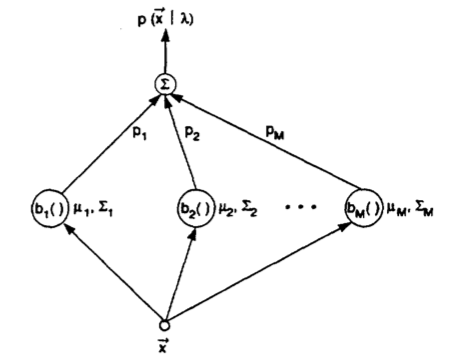
\includegraphics[width=0.5\textwidth]{figures/gmm_structure.png}
            \caption{Visualization of a GMM. The Gaussian mixture is the weighted sum of several Gaussian distributions, where $p_i$ are the mixture weights and $b_i$ are the Gaussians. \cite{reynolds_rose}}
            \label{fig:gmm_structure}
        \end{center}
    \end{figure}

    % \begin{figure}
    %     \begin{center}
    %         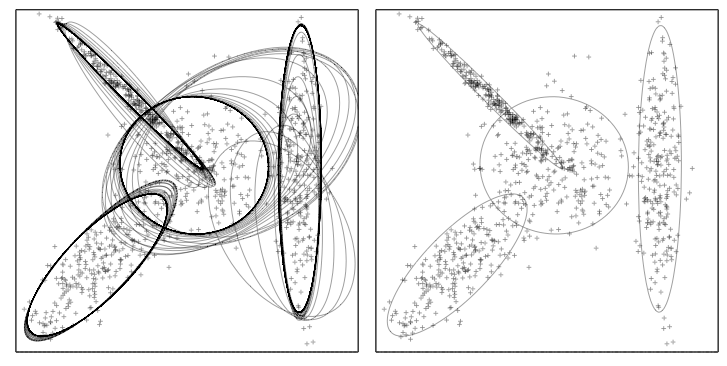
\includegraphics[width=1\textwidth]{figures/gmm_training.png}
    %         \caption{Example of a GMM in two dimensions. Crosses signify the data points, ellipses the three multivariate Gaussians. On the left-hand side, the evolution of the estimated means and covariances of these Gaussians during the EM process is shown;  the right-hand side shows the converged mixture. \cite{numerical_recipes}}
    %         \label{fig:gmm_training}
    %     \end{center}
    % \end{figure}

    Gaussian Mixture Models have been used in many areas of machine learning, for example in ASR \cite{reynolds_rose}, in image retrieval \cite{permuter}, in financial modeling \cite{alexander}, and in visual tracking \cite{chen_adebomi}. 
    When used for classification, one GMM is trained for each class $S = (s_1, s_2, ..., s_J)$ separately, resulting in $J$ sets of parameters $\lambda$. 
    The likelihood $L_j$ of each class is then determined, and the most likely class is chosen:

    \begin{equation}
        C = \argmax_{1 \leq j \leq J } P(\lambda_j | X) = \argmax_{1 \leq j \leq J} \frac{p(X | \lambda_j) P(\lambda_j)}{p(X)}
    \end{equation}

    
    If all classes and all observations are equally likely, this simplifies to

    \begin{equation}
        C = \argmax_{1 \leq j \leq J } p(X | \lambda_j) 
    \end{equation}

    In practice, log-probabilities are commonly used for numerical reasons, resulting in the calculation:

    \begin{equation}
        C = \argmax_{1 \leq j \leq J} \sum_{n=1}^N \log p(x_n | \lambda_j)
    \end{equation}

    In addition to this direct use for classification, GMMs are often used to model the emission probabilities in Hidden Markov Models, these are then called GMM-HMMs.